\clearpage\section{Chapter 6: Databases}

\index{database}Databases are technically part of the system interface
described in the last chapter, but they are an important application
area in their own right. There are different kinds of databases, and
the appropriate database to use depends on how much information is to
be stored, and what kinds of accesses to the information are supported.
This chapter describes three database mechanisms for which Unicon
provides direct support. In this chapter you will learn how to:

\begin{itemize}
\item Read and write memory-based structures to data files.
\item Use DBM databases as a persistent table data type.
\item Manipulate SQL databases through the ODBC connection mechanism.
\end{itemize}
\subsection{Language Support for Databases}
Unicon provides transparent access to databases stored in local files
and on remote servers. The term
{\textquotedbl}transparent{\textquotedbl} means that the built-in
functions and operators used to access information in a database are
the same as those used to access information in the memory-based
structures presented in Chapter 2. To do this, connections to databases
are represented by new built-in types that are extensions of the file
and table data types.

Some people might prefer a different syntax for databases from what is
used for data structures. A different syntax, such as one based purely
on function calls, would be consonant with the difference in
performance the programmer can expect to see when accessing data in
files as opposed to memory-based data structures. However, the
performance of operators already depends on the type of the operands.
Consider the expression \textsf{!x}. If \textsf{x} is a structure, its
elements are generated from memory, but if \textsf{x} is a file,
\textsf{!x} reads and generates lines from the file. The goal for
Unicon is to make databases just as easy to learn and use as the rest
of the language, and to minimize the introduction of new concepts.

The word {\textquotedbl}database{\textquotedbl} means different things
to different people. For some, the term is used as the short form of
the term {\textquotedbl}relational database.{\textquotedbl} This
chapter uses the term database to refer to any method of providing
{\textquotedbl}persistent structures{\textquotedbl} that store
information from one program run to the next. The operators that are
used to access a database determine whether a single element at a time
is read or written, or whether many operations are buffered and sent to
the database together.

\subsection{Memory-based Databases}
Some people would not consider a memory-based
\index{database!in-memory}database to be a database at all. If the
entire database fits in memory at once, you can generally achieve vast
speedups by avoiding the disk as much as possible. For example, all
forms of querying or reading the database can be performed from memory.
The database may be modified in memory immediately, and updated on the
disk later on. Memory-based databases were limited in value ten years
ago, but in the age where a gigabyte of main memory for your PC is
affordable, they may be the best choice for many or most applications.

One easy way to implement a memory-based database is to build up your
arbitrary structure in memory, and then use the Icon Program Library
procedures in module \textsf{xcodes} to write them out and read them
in. The \index{xcodes}\textsf{xcodes} procedures flatten structures
into a canonical string format that can be written to a file, and
convert such strings back into the corresponding structure. If variable
\textsf{db} contains such a structure, the following sequence saves the
contents of \textsf{db} to a file named \textsf{db.dat.}

\iconcode{
db := table() \\
db[{\textquotedbl}Ralph{\textquotedbl}] :=
{\textquotedbl}800-USE-ICON{\textquotedbl} \\
db[{\textquotedbl}Ray{\textquotedbl}] :=
{\textquotedbl}800-4UN-ICON{\textquotedbl} \\
dbf :=
open({\textquotedbl}db.dat{\textquotedbl},{\textquotedbl}w{\textquotedbl}) \\
xencode(db, dbf) \\
close(dbf)
}

\noindent
The converse operation, reading in a structure from a file is also
simple:

\iconcode{
dbf := open({\textquotedbl}db.dat{\textquotedbl}) \\
db := xdecode(dbf) \\
close(dbf) \\
write(db[{\textquotedbl}Ralph{\textquotedbl}])
}

This approach works great for databases that do not need to be written
to disk on an on-going basis and for which the queries can readily be
expressed as operations on structure types. For example, a telephone
rolodex application would be well-served by this type of database. The
data fits comfortably in memory, updates often occur in batches, and
simple queries (such as a student{\textquotesingle}s name) provide
sufficient access to the data. The other two kinds of databases in this
chapter use traditional database technologies to efficiently address
situations where this type of database is inadequate.

\subsection{DBM Databases}

A classic database solution on the UNIX platform is provided by the DBM
family of library functions. \index{DBM}DBM stands for Data Base
Manager, and the functions maintain an association between keys and
values on disk, which is very similar to the table data type. DBM was
eventually followed by compatible superset libraries called NDBM (New
Data Base Manager) and GDBM (GNU Data Base Manager). Unicon uses GDBM
on all platforms.

DBM databases are opened by the \textsf{open()} function using mode
\textsf{{\textquotedbl}d{\textquotedbl}}. By default, a database is
opened for reading and writing; mode
\textsf{{\textquotedbl}dr{\textquotedbl}} opens a database read-only.
Once opened, DBM databases are treated as a special case of the table
data type and are manipulated using table operations. For example, if
\textsf{d} is a DBM file, \textsf{d[s]} performs a database
insert/update or lookup, depending on whether the expression is
assigned a new value, or just \index{dereference}dereferenced for its
current value. For persons who do not like to use \index{subscript
operator}subscript operators for everything, values can also be
inserted into the database with \index{insert()!DBM
database}\textsf{insert(d, k, v)} and read from it with
\index{fetch()!DBM database}\textsf{fetch(d, k)}. \index{delete()!DBM
database}\textsf{delete(d, k)} similarly deletes key \textsf{k} from
the database. DBM databases are closed using the \textsf{close()}
function. The following example program takes a database and a key on
the command line, and writes out the value corresponding to that key.

\iconcode{
procedure main(args) \\
\>   d := open(args[1], {\textquotedbl}d{\textquotedbl}) {\textbar}
stop({\textquotedbl}can{\textquotesingle}t open {\textquotedbl},
args[1]) \\
\>   write(d[args[2]]) \\
end
}

If you are wondering why the call to \textsf{open()}
isn{\textquotesingle}t followed by a call to \textsf{close()}, you are
right, it is proper to close files explicitly, although the system
closes all files when the program terminates. How would you generalize
this program to accept a third command-line argument, and insert the
third argument (if it is present) into the database with the key given
by the second argument? You might easily wind up with something like
this:

\iconcode{
procedure main(args) \\
\>   d := open(args[1], {\textquotedbl}d{\textquotedbl}) {\textbar}
stop({\textquotedbl}can{\textquotesingle}t open {\textquotedbl},
args[1]) \\
\>   d[args[2]] := args[3] \\
\>   write(d[args[2]]) \\
\>   close(d) \\
end
}

DBM databases are good for managing data sets with a simple
organization, when the size of the database requires that you update
the database a record at a time, instead of writing the entire data
set. For example, if you wrote a Web browser, you might use a DBM
database to store the user{\textquotesingle}s set of bookmarks to Web
pages of interest. In fact, Netscape uses DBM files for its bookmarks.

There is one basic limitation of DBM databases when compared with the
table data type that you should know about. DBM databases are
string-based. The keys and values you put in a DBM database get
converted and written out as strings. This makes the semantics of DBM
databases slightly different from tables. For example, a table can have
two separate keys for the integer \textsf{1} and the string
\textsf{{\textquotedbl}1{\textquotedbl}}, but a DBM database will treat
both keys as the string \textsf{{\textquotedbl}1{\textquotedbl}}. This
limitation on DBM databases also means that you cannot use structure
types such as lists as keys or values in the database. If the type is
not convertible to string, it won{\textquotesingle}t work. You can use
the functions \textsf{xencode()} and \textsf{xdecode()}, described in
the previous section, to manually convert between strings and
structures for storage in a DBM database if you really need this
capability.

\subsection[SQL Databases]{SQL Databases}

\index{SQL}DBM is great for data that can be organized around a single
key, but it is not much help for more complex databases. The industry
standard choice for enterprise-level data organization is the
Structured Query Language (SQL). SQL is supported by every major
database vendor.

A SQL database is more complex than a DBM database. It can contain
multiple tables, and those tables are accessed by walking through a set
of results to a query, rather than by accessing individual elements
directly. SQL is designed for industrial-strength relational databases.

\subsubsection{The SQL Language}

The SQL language was invented by IBM and based on relational database
theory developed by E.F. Codd. A database is a collection of
\textit{tables}, and each table is a collection of \textit{rows}. The
rows in a table contain information of various types in a set of named
\textit{columns}. Rows and columns are similar to records and fields,
except that they are logical structures and do not describe physical
form or layout of the data. There is an ANSI standard definition of
SQL, but many vendors provide extensions, and most vendors are also
missing features from the ANSI standard. Unicon allows you to send any
string you want to the SQL server, so you can write portable
{\textquotedbl}vanilla SQL{\textquotedbl} or you can write
vendor-specific SQL as needed.

SQL was originally intended for text-based interactive sessions between
humans and their databases, but is now primarily used
{\textquotedbl}under the covers{\textquotedbl} by database
applications. Many database applications accommodate novice users with
a graphical interface that does not require any knowledge of SQL, while
supporting a SQL {\textquotedbl}escape hatch{\textquotedbl} for
advanced users who may wish to do custom queries. This duality is
paralleled in the Unicon language by the fact that
Unicon{\textquotesingle}s built-in database operators and functions
duplicate a subset of the capabilities of SQL. There are two ways to do
things: using Unicon operations or using SQL statements.

SQL statements can be divided into several categories, the most
prominent of which are data definition and data manipulation. When
using SQL within a Unicon program, you build up string values
containing SQL statements. In the following examples, the SQL is given
unadorned by double quotes or other Unicon artifacts.

New tables are created with a \textsf{CREATE TABLE} statement, such as

\iconcode{
create table addresses (name varchar(40), address varchar(40), phone
varchar(15))}

Tables have a primary key, which must be unique among rows in the table.
By default the primary key is the first one listed, so \textsf{name} is
the primary key in table \textsf{addresses} above.

SQL{\textquotesingle}s data manipulation operations include
\textsf{SELECT}, \textsf{INSERT}, \textsf{UPDATE}, and \textsf{DELETE}.
\textsf{SELECT} allows you to refine the data set being operated on,
picking rows and columns that form some projection of the original
table. Perhaps more importantly, \textsf{SELECT} allows you to combine
information from multiple tables using relational algebra operations.
Most databases are long-lived and evolve to include more columns of
information over time. SQL{\textquotesingle}s ability to select and
operate on projections is an important feature, since code that works
with a certain set of columns continues to work after the database is
modified to include additional columns.

\textsf{INSERT}, \textsf{UPDATE}, and \textsf{DELETE} all modify the
table{\textquotesingle}s contents. \textsf{INSERT} adds new rows to a
table. \ For example:

\iconcode{
insert into addresses (name, address, phone) \\
\>   \ \ \ \ values ({\textquotesingle}Nick K{\textquotesingle},
{\textquotesingle}1 Evil Empire{\textquotesingle},
{\textquotesingle}(123)456-7890{\textquotesingle}) \\
insert into addresses (name, address, phone) \\
\>   \ \ \ \ values ({\textquotesingle}Vic T{\textquotesingle},
{\textquotesingle}23 Frozen Glade{\textquotesingle},
{\textquotesingle}(900)888-8888{\textquotesingle})
}

\textsf{UPDATE} and \textsf{DELETE} can modify or remove sets of rows
that match a particular criterion, as in

\iconcode{
update addresses set address = {\textquotesingle}666 RTH,
Issaquah{\textquotesingle} \\
\>   \ \ \ \ \ \ \ \ \ \ \ \ \ \ where name = {\textquotesingle}Nick
K{\textquotesingle} \\
delete from addresses where name = {\textquotesingle}Vic
T{\textquotesingle}
}

This section presented only a few aspects of the SQL language. For
simple database tasks you can in fact ignore SQL and use the Unicon
facilities described in the rest of this chapter. However, for more
complex operations the best solution is to formulate some SQL commands
to solve the problem. A full discussion of SQL is beyond the scope of
this book. For more information on this topic you might want to read
one of the following books: Ramez Elmasri and Shamkant
Navanthe{\textquotesingle}s \textit{Fundamentals of Database Systems,}
C.J. Date and Hugh Darwen{\textquotesingle}s \textit{A Guide to the SQL
Standard}.

\subsubsection[Database Architectures and ODBC]{Database Architectures
and ODBC}

\index{ODBC}SQL databases are accessed through an underlying Open
DataBase Connectivity (ODBC) transport mechanism. This mechanism allows
the programmer to ignore the underlying architecture. Hiding this
complexity from application programmers is important. The database
architecture may vary from a single process accessing a local database,
to client/server processes, to three or more tiers spanning multiple
networks. Figure 6-1 illustrates the role played by ODBC in providing
Unicon with database access in one- and two-tier configurations. While
this chapter cannot present a complete guide to the construction of
database systems, it provides concrete examples of writing Unicon
client programs that access typical database servers.

\begin{center}
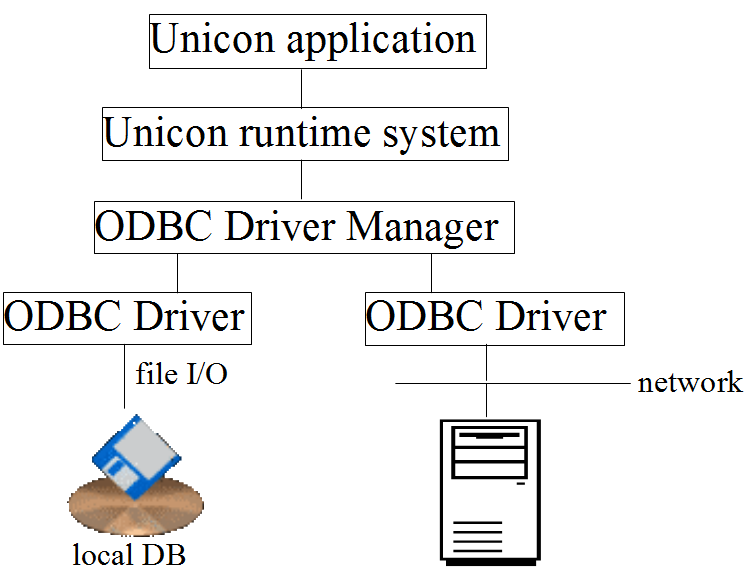
\includegraphics[width=4in,height=3in]{ub-img/odbcarch.png}
\end{center}

{\sffamily\bfseries Figure 6-1:}
{\sffamily ODBC hides database architecture; Unicon hides ODBC from
 applications}

\bigskip

To use Unicon{\textquotesingle}s SQL facilities, you must have several
software components in place. First, you need a SQL server that
supports ODBC. You could buy a commercial SQL server, or you may be
able to use a free or low-cost server such as \index{MySQL}MySQL
(\textsf{www.mysql.com}) or \index{PostgreSQL}PostgreSQL
(\textsf{www.postgresql.org}).

Second, you need an account, password, and permissions on the SQL
server, so that you can connect to it. The details of this process are
necessarily server-dependent and unfortunately outside the scope of
this book.

Third, your client machine needs an \index{driver manager!ODBC}ODBC
driver manager, and an ODBC driver for your SQL server, and these have
to be configured properly. The driver manager is a piece of system
software that multiplexes applications to different databases, while
the drivers are the dynamic link libraries that database vendors supply
to talk to their database. Once you have the ODBC software set up,
writing the Unicon client program to connect to your database is
straightforward.

\subsubsection[Opening a SQL Database]{Opening a SQL Database}
Connecting to a SQL database is performed by calling \textsf{open()}
with mode \textsf{{\textquotedbl}o{\textquotedbl}}. This establishes a
session with a data source. The filename argument to \textsf{open()} is
the data source to which you are connecting; it is associated with a
particular ODBC driver, remote database server machine or IP number,
and port within the ODBC driver manager. Mode
\textsf{{\textquotedbl}o{\textquotedbl}} uses additional arguments to
\textsf{open()} that specify the user name and password to use in
connecting to the specified data source. Here is an example that
establishes a connection to a database:

\iconcode{
f := open({\textquotedbl}unicondb{\textquotedbl},
{\textquotedbl}o{\textquotedbl}, {\textquotedbl}scott{\textquotedbl},
{\textquotedbl}tiger{\textquotedbl})}

The \textsf{open()} function returns a value that supports many of the
operations of both a file and a table. If the connection
can{\textquotesingle}t be established, the call fails. The underlying
session information is maintained separately and may be shared by
multiple calls to \textsf{open()} to the same database. In addition to
the network connection and SQL session information that is retained,
each database file value maintains a current \textit{selection}
consisting of a set of rows corresponding to the current query, and a
\textit{cursor position} within that selection. When a database is
first opened, the selection consists of a null set containing no rows
and no columns.

\subsubsection{Querying and Modifying a SQL Database}
Subsequent queries to the database can be made by calling
\textsf{sql(db, sqlcmd)}. The \index{sql()}\textsf{sql()} function sets
the current selection within the database and places the cursor at the
beginning of the set of selected rows. For example, to obtain Vic
T{\textquotesingle}s phone number you might say

\iconcode{
sql(f, {\textquotedbl}select phone from addresses where
name={\textquotesingle}Vic T{\textquotesingle}{\textquotedbl})}

Vic{\textquotesingle}s phone number is included if you use the original
\textsf{select *} query, but the more specific your query, the less
time and network bandwidth is wasted sending data that your client
application must filter out. You should do as much work on the server
(in SQL) as possible to make the client more efficient.

Since the function \textsf{sql()} transmits arbitrary SQL statements to
the server, it can be used for many operations besides changing the
current selection. The \textsf{sql()} function returns a null value
when there is no return value from the operation, such as a
\textsf{create table} statement. Its return value can be of varying
type for other kinds of queries, and it can fail, for example if the
SQL string is malformed or requests an impossible operation.

\subsubsection{Traversing the Selected Rows}
To walk through the rows of your current database selection, you call
\index{fetch()!SQL}\textsf{fetch(db)}. The value returned is a
\textit{row} that has many of the operations of a record or a table,
namely field access and subscripting operators. For example, if
\textsf{fetch(db)} returns a row containing columns Name, Address, and
Phone, you can write

\iconcode{
row := fetch(db) \\
write(row.Name) \\
write(row[{\textquotedbl}Address{\textquotedbl}])
}

Called with one argument, \textsf{fetch(db)} moves the cursor forward
one position. With two arguments, \textsf{fetch(db, column)} fetches a
single column from the current row, without advancing the cursor.

\subsubsection[A SQL Example Application]{A SQL Example Application}
\index{SQL}A human resources database might include two tables. One
table might maintain employee information, such as names,
identification numbers, and phone numbers, while another table
maintains entries about specific jobs held, including
employee{\textquotesingle}sID, the pay rate, a code indicating whether
pay is hourly or salaried, and the job title. Note that the SQL is
embedded within a string literal.

\iconcode{
sql(db, {\textquotedbl}create table employees (id varchar(11), name
varchar(40), phone varchar(15)){\textquotedbl}) \\
sql(db, {\textquotedbl}create table jobs (id varchar(11), payrate
integer, is\_salaried char, title varchar(40)){\textquotedbl})
}

\noindent
Inserting rows into the database looks like

\iconcode{
sql({\textquotedbl}insert into employees (id, name, phone) values(32,
{\textquotesingle}Ray{\textquotesingle},
{\textquotesingle}274-2977{\textquotesingle}){\textquotedbl})}

Now, how can you print out the job title for any particular employee? If
you have the employee{\textquotesingle}s identification number, the
task is easy, but let{\textquotesingle}s say you just have their name.
These are the kinds of jobs for which SQL was created. Information from
the employees table is effortlessly cross-referenced with the jobs
table by the following SQL. \ The string is long so it is split into
two lines. A Unicon string literal spans multiple lines when the
closing doublequote has not been found and the line ends with an
underscore character.

\iconcode{
sql(db, {\textquotedbl}select name,title from employees,jobs \_ \\
\>   \ \ \ \ \ \ where name={\textquotesingle}Ray{\textquotesingle} and
employees.id = jobs.id{\textquotedbl}) \\
while write(fetch(db).Title)
}

\subsubsection{SQL Types and Unicon Types}

SQL has many data types, most of which correspond well to Unicon types.
For example, \textsf{CHAR} and \textsf{VARCHAR} correspond to Icon
strings, \textsf{INTEGER} and \textsf{SMALLINT} correspond to integers,
\textsf{FLOAT} and \textsf{REAL} correspond to reals, and so on. The
philosophy is to convert between Icon and SQL seamlessly and with
minimal changes to the data format, but you should be aware that these
are not exact matches. For example, it is possible to define a
\textsf{FLOAT} with more precision than an Icon real, and it is easy to
produce an Icon string that is longer than the maximum allowed
\textsf{VARCHAR} size on most SQL servers. Unicon programmers writing
SQL clients must be aware of the limitations of the SQL implementations
they use.

Unicon has structure types for which there is no SQL equivalent. Values
of these types cannot be inserted into a SQL database unless you
explicitly convert them to a SQL-compatible type (usually, a string)
using a function such as \textsf{xencode()}.

SQL also has types not found in Unicon. These types, such as bit
strings, datetimes, timestamps, and BLOBS, are generally all
represented by strings, and strings are used to insert such values into
SQL databases. In fact, strings are the {\textquotedbl}magic
fingers{\textquotedbl} of the whole interface, since they are also the
type used by the system to represent out of range values when reading
SQL columns into Unicon. But, you are probably tired of me stringing
you along about databases by now.

\subsubsection{More SQL Database Functions}

SQL databases are complicated enough, and feature-rich enough to warrant
their own repertoire of functions in addition to the operations they
share with other kinds of files and databases. These functions are
described in detail in Appendix A, but a few of them deserve special
mention. The function \textsf{dbtables(db)} is useful to obtain a
listing of the data sources available within a particular database.
Function \textsf{dbcolumns(db)} provides detailed information about the
current table that is useful in writing general tools for viewing or
modifying arbitrary SQL databases.

The functions \textsf{dbproduct(db)} and \textsf{dbdriver(db)} produce
information about the DBMS to which db is connected, and the
\index{ODBC}ODBC driver software used in the connection, respectively.
The function \textsf{dblimits(db)} produces the upper bounds for many
DBMS system parameters, such as the maximum number of columns allowed
in a table. All three of these functions return their results as either
a record or list of records; the record field names and descriptions
are given in Appendix A.

\subsection{Tips and Tricks for SQL Database Applications}

In addition to the complexity of learning SQL itself, SQL database
applications have a characteristic flavor which may or may not seem
natural to the Unicon programmer.

\subsubsection{Operating on Large Files}

If anything can bring a modern workstation to its knees, it is asking
for 200MB of data in a remote SQL database. Some SQL operations are
slow due to an inefficient query on the remote server, while others are
slow because large amounts of data are transmitted over a limited
network connection. For a fixed amount of data, operation time will
vary radically depending on how it is organized; fewer, larger tuples
are transmitted faster than many smaller tuples.

\subsubsection{Use Multiple Connections to Nest Queries}

It is common to use more than one table at once. Some times this is
using SQL{\textquotesingle}s \textsf{JOIN} operation, but sometimes it
is not. If you try to nest a second query inside a first one, you will
quickly find that on a given connection, only one \textsf{SELECT} and
one row set is maintained at a time. The second \textsf{SELECT}
replaces the first, so for example:

\iconcode{
db := open({\textquotedbl}mydsn{\textquotedbl},
{\textquotedbl}o{\textquotedbl}, ...) \\
sql(db, {\textquotedblleft}SELECT ...{\textquotedblright}) \\
while r := fetch(db) do \{ \\
\>   sql(db, {\textquotedblleft}SELECT ...{\textquotedblright}) \\
\>   while r2 := fetch(db) do write(r2.foo) \\
\>   \}
}

\noindent
does not work. Within your operating system and database
server{\textquotesingle}s limits, the easy solution is to open multiple
connections to your database:

\iconcode{
db1 := open({\textquotedbl}mydsn{\textquotedbl},
{\textquotedbl}o{\textquotedbl}, ...) \\
db2 := open({\textquotedbl}mydsn{\textquotedbl},
{\textquotedbl}o{\textquotedbl}, ...) \\
sql(db, {\textquotedblleft}SELECT ...{\textquotedblright}) \\
while r := fetch(db) do \{ \\
\>   sql(db2, {\textquotedblleft}SELECT ...{\textquotedblright}) \\
\>   while r2 := fetch(db2) do write(r2.foo) \\
\>   \}
}

\subsubsection{Dynamic Records}

You may be wondering exactly how rows are represented. Actually, they
are records, but their fields are determined at run-time from the names
of selected columns. Such new record types that are introduced on the
fly are called \textit{dynamic records}, and they are useful in other
contexts besides databases.

The function \index{constructor!dynamic record
type}\textsf{constructor(recordname, field, field, ?)} produces a
Unicon record constructor procedure for records named
\textsf{recordname} with the specified fields. The fields of dynamic
records can be arbitrary strings, not just legal identifiers, but
obviously the field operator (\textsf{.}) cannot be used for fields
that are not identifiers.

\subsubsection[The db Library]{The \texttt{db} Library}
By adding \textsf{link db} to your program you can access a library that
provides simplified access to SQL databases for non-SQL programmers.
These procedures will not spare you the pain of learning SQL for long,
but may ease the conversion from Unicon structure values into SQL
strings for transmission over the network.

The most useful of these procedures is \textsf{dbupdate()}, which sends
a record (tuple) to the database. The following example updates two
columns within a row returned by \textsf{fetch()}.

\iconcode{
row := fetch(db) \\
row.Name := {\textquotedbl}Bill Snyder{\textquotedbl} \\
row[{\textquotedbl}Address{\textquotedbl}] := {\textquotedbl}6900
Tropicana Blvd{\textquotedbl} \\
dbupdate(db, row)
}

Of course, before a fetch can be performed, a row set must have been
selected. The procedure \textsf{dbselect(db, columns, filter, order)}
selects tuples containing columns from the database, with optional
filter(s) and ordering rule(s).

Inserting and deleting rows may be performed by the procedures
\textsf{dbinsert()} and \textsf{dbdelete()}. The \textsf{dbinsert()}
function takes two parameters for each column being inserted, the
column name and then the value.

\subsubsection{Unwritable Tuples}
It is worth mentioning that many forms of SQL selections are read-only.
The relational combination of columns from different tables is a
powerful abstraction, but the resulting selections are non-updatable.
Another example of a read-only query is a \textsf{GROUP BY} query,
which is usually applied before an aggregate count. Executing a
\textsf{SELECT *} on a single table is guaranteed to be updatable, but
if you do something fancier, you will have to know the semantics of SQL
to tell whether the result may be modified.

{\sffamily
Summary}

Databases are a vital form of persistent storage for modern
applications. The notation used to manipulate a database can look like
a sequence of table and record operations, or it may be an obvious
combination of Unicon and SQL statements. Either way, database
facilities give programmers more direct access and control over the
information flow to and from permanent storage.


\bigskip

